\clearpage
\section{Vesture and Ministry Distinctions}
Diversity of vestments outwardly manifests the diversity of ministries within Christ's Body (GIRM 335). Every minister---bishop, priest, deacon, instituted acolyte, instituted lector, extraordinary minister of Holy Communion, and altar server---wears attire proper to that office, and lay ministers never assume the stole, dalmatic, or chasuble reserved to Holy Orders (Redemptionis Sacramentum 126).

\subsection*{Distinct Ministers in the Postconciliar Sanctuary}
The General Instruction of the Roman Missal distinguishes ordained ministers, instituted lay ministries, extraordinary ministers of Holy Communion, and altar servers. Each office carries its own vesture and handling boundary, and none is interchangeable with another.

{\footnotesize\begin{longtable}{>{\raggedright\arraybackslash}p{0.20\linewidth}>{\raggedright\arraybackslash}p{0.28\linewidth}>{\raggedright\arraybackslash}p{0.45\linewidth}}
\toprule
\textbf{Minister} & \textbf{Appointed vesture} & \textbf{Sanctuary and handling role} \\
\midrule
\endhead
\textbf{Bishop (Episcopus)} & Alb, cincture, amice (if needed), pectoral cross, straight stole, pontifical dalmatic (at major pontifical Masses), chasuble or cope, miter, ring, crosier. & Principal liturgist of the diocese (GIRM 92); dedicates fixed altars, consecrates Sacred Chrism, blesses Holy Oils, judges tabernacle placement (GIRM 315), ordinary minister of Holy Communion. \\
\textbf{Priest (Presbyter)} & Alb, cincture (unless fitted), amice (if collar exposed), straight vertical stole, chasuble at Mass (GIRM 337); cope outside Mass (GIRM 341); choir dress or cassock and surplice when not concelebrating (RS 128). & Confects the Eucharist in the person of Christ the Head (GIRM 93; RS 154); blesses vessels and vestments (GIRM 333, 335); ordinary minister of Holy Communion; consumes remaining Precious Blood and purifies sacred vessels. \\
\textbf{Deacon (Diaconus)} & Alb, cincture (unless fitted), amice (if collar exposed), diagonal stole over left shoulder fastened at right hip (GIRM 340), dalmatic worn over stole (GIRM 338; omission discouraged by RS 125). & Carries Book of the Gospels and proclaims Gospel; prepares altar and chalice; elevates chalice at doxology; ordinary minister of Holy Communion and especially of the chalice (GIRM 182); purifies vessels (GIRM 279). \\
\textbf{Instituted Acolyte (Acolythus institutus)} & Alb (common garment of instituted ministers, GIRM 336) or other dignified attire in U.S. (GIRM 339); never stole, dalmatic, or chasuble (RS 126). & Layperson formally instituted by the bishop (Ministeria quaedam 1972; CIC can. 230 as amended by Spiritus Domini 2021). Assists at altar; extraordinary minister of Holy Communion ex officio; uniquely among laity may purify sacred vessels (GIRM 279; USCCB Norms 53). \\
\textbf{Instituted Lector (Lector institutus)} & Alb (GIRM 336) or dignified attire in U.S. (GIRM 339); never stole, dalmatic, or chasuble (RS 126). & Layperson formally instituted by the bishop (CIC can. 230). Carries Book of the Gospels in entrance procession only in the deacon's absence (GIRM 120d, 194); proclaims Scripture readings other than the Gospel and intentions of Universal Prayer. \\
\textbf{Extraordinary Minister of Holy Communion (EMHC)} & Dignified lay attire or alb per diocesan directive (GIRM 339); never clerical vestments or stole (RS 126). & Deputed layperson acting strictly in genuine pastoral necessity (GIRM 100, 162; RS 155--158). Approaches altar only after the priest communicates (USCCB Norms 38); distributes Communion from handed vessels; may not purify sacred vessels (GIRM 279; Oct 2006 CDWDS decision; USCCB Norms 53). \\
\textbf{Altar Server (Ministrans)} & Alb (with cincture if unfitted) or black cassock with white surplice (never surplice without cassock, CE 65) or other dignified attire approved in U.S. (GIRM 339); never clerical insignia. & Non-instituted lay server (GIRM 107; RS 47). Carries processional cross, candles, thurible, boat, bells, cruets, lavabo, and aspersorium; holds Missal or Book of the Chair; brings unconsecrated vessels at Preparation of Gifts. Never opens tabernacle, carries consecrated species, carries Book of Gospels in procession, or purifies vessels. \\
\textbf{Sacristan (Sacrista)} & Ordinary dignified attire in the sacristy (vested in alb or cassock and surplice only when also exercising a sanctuary ministry). & Prepares sacred vessels, linens, liturgical books, vestments, candles, and credence table before Mass and sees to orderly care, sacrarium first-rinsing of linens (RS 120), and storage after Mass (GIRM 105). \\
\bottomrule
\end{longtable}}

\clearpage
\subsection{Ordained Vesture at Mass}
\PCDPlateHeader{Plate VIII --- Ordained Vesture at Mass}{Standing figures to common scale; insets not to scale}
\ifdefined\TriptychPrintEdition
\begin{center}
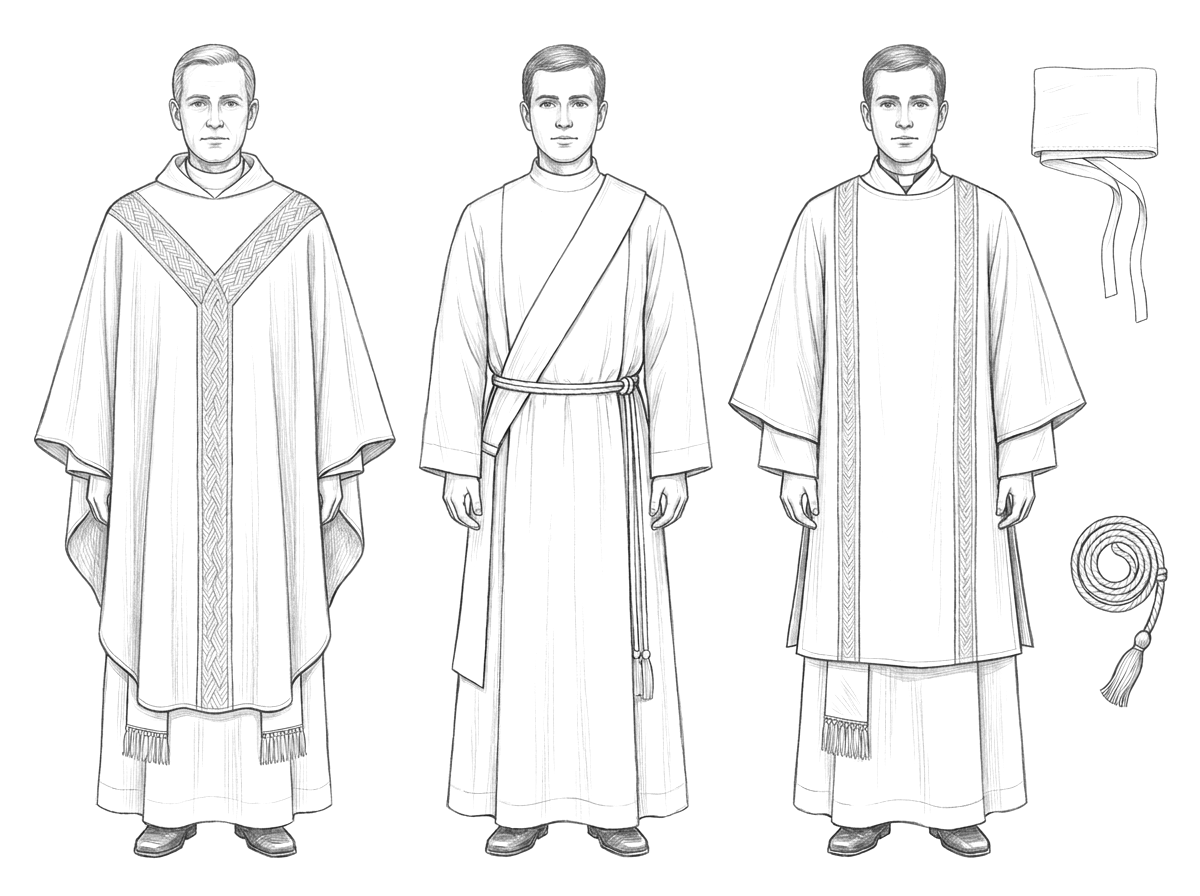
\includegraphics[width=0.92\linewidth,height=3.55in,keepaspectratio]{liturgy/roman-rite/postconciliar/2008-latin-2011-us-english/reference/roman-sanctuary-dictionary/shared/artwork/graphite/pc-art-08-priest-deacon-vesture.png}
\end{center}
\PCDPositionKey{Left: Priest in Alb, Amice, straight vertical Stole, and Y-orphrey Chasuble; center: Deacon in Alb, Cincture, and diagonal Stole from left shoulder to right hip without dalmatic; right: Deacon in Alb and sleeved Dalmatic worn over the diagonal Stole (fringed tip peeking at deacon's right side); far right insets: folded Amice with ties (top) and coiled tasseled Cincture (bottom).}
\else
\textbf{Visual Plate Summary (Plate VIII --- Ordained Vesture at Mass, Standing figures to common scale; insets not to scale):} Worn monochrome graphite vestment study comparing priest and deacon at common scale: left, a priest vested in ankle-length white alb, amice at collar, straight vertical stole ends visible below a flowing Gothic chasuble with Y-shaped orphrey; center, a deacon in white alb and tied cord cincture wearing his stole diagonally from left shoulder across the chest to his right hip; right, a deacon vested in a wide-sleeved dalmatic with vertical clavi stripes worn over the diagonal stole, whose fringed end peeks below the deacon's right hem; far right margin insets show a folded rectangular amice with cloth ties above and a coiled tasseled cincture below.

\textbf{Reading order and object placement:} Left: Priest in Alb, Amice, straight vertical Stole, and Y-orphrey Chasuble; center: Deacon in Alb, Cincture, and diagonal Stole from left shoulder to right hip without dalmatic; right: Deacon in Alb and sleeved Dalmatic worn over the diagonal Stole (fringed tip peeking at deacon's right side); far right insets: folded Amice with ties (top) and coiled tasseled Cincture (bottom).
\fi

\label{pc-obj-alb}
\PCDEntryHead{Alb}{Alba}{required}{N31}
\PCDField{Also called}{White Tunic; \textit{Tunica alba}}
The alb is the full-length white liturgical tunic that serves as the common sacred garment of all ordained and instituted ministers of every rank. Cut to ankle length with full-length sleeves in plain white linen or woven fabric, the alb appears beneath the priest's chasuble, the center deacon's diagonal stole and cincture, and the right deacon's dalmatic in Plate VIII, as well as under the cope and humeral veil in Plate IX.

\PCDField{Plate position and status}{Worn beneath chasuble, diagonal stole, and dalmatic across all three figures (Plate VIII), and under cope and humeral veil (Plate IX) (Universal Roman law)}
\PCDField{Placement and liturgical use}{Under universal Roman law, bishops, priests, deacons, instituted acolytes, and instituted lectors wear the alb as their shared liturgical garment (GIRM 336; RS 121--122). It is tied at the waist with a cincture unless tailored to fit neatly without one, and preceded by an amice whenever its neckline leaves ordinary clothing visible at the collar (GIRM 336; Caeremoniale Episcoporum 65). A surplice---even worn over a cassock---may never be substituted for the alb when a chasuble, a dalmatic, or a stole alone is worn (GIRM 336). In the United States, altar servers, readers, and extraordinary ministers of Holy Communion may wear the alb or other dignified clothing approved by diocesan norm (US GIRM 339), but lay ministers never add a stole, dalmatic, or chasuble over it (RS 126).}
\PCDField{United States norm}{While GIRM 336 establishes the alb universally for all ordained and instituted ministers, the USCCB adaptation at GIRM 339 permits acolytes, altar servers, readers, and other lay ministers in the Dioceses of the United States to wear either the alb or other dignified attire suited to liturgical service.}
\PCDField{Ministers and server boundary}{Ordinary ministers: Bishop, Priest, Deacon, Instituted acolyte, Instituted lector, Extraordinary minister of Holy Communion, Altar server. Server handles directly: Altar servers may wear a clean white alb hemmed at ankle height (tied with a cincture if unfitted) where parish custom appoints it under US GIRM 339, hanging it neatly after Mass and never wearing clerical insignia over it (RS 126).}
\PCDSafety{Choose an alb whose hem clears your shoes cleanly at ankle height; an overly long hem catches on sanctuary steps and creates a serious tripping hazard, especially when carrying lighted candles, cruets, or a hot thurible.}
\PCDField{Distinguish from}{Cassock and Surplice}
\PCDField{Symbolism}{As the single white garment shared by ordained and instituted ministers of every rank, the alb outwardly recalls baptismal dignity in Christ (GIRM 335--336), echoing St. Paul, ``For as many of you as have been baptized in Christ have put on Christ'' (Gal 3:27), and the saints who ``have washed their robes and have made them white in the blood of the Lamb'' (Apoc 7:14). Outside the norms of the General Instruction, the traditional Roman sacristy vesting prayer asks the Lord to make the minister pure and white in the blood of the Lamb, and Amalarius of Metz interprets the loose linen tunic as Christian freedom and bodily discipline. (GIRM 335--336; Gal 3:27; Apoc 7:13--14; traditional Roman sacristy vesting prayer (Ad Albam); Amalarius of Metz, Liber Officialis II.18)}
\PCDField{1962 Roman Missal counterpart}{\PCDTag{changed use} In the 1962 Roman Missal, the alb was worn solely by ordained sacred ministers at Mass (bishop, priest, deacon, and subdeacon, RS I.2--3), while altar servers and minor clerics wore cassock and surplice (RS II.1, VI.8). Under the 2002/2008 GIRM, the alb becomes the universal common garment of all ordained and instituted ministers, may never be replaced by a surplice under a chasuble, dalmatic, or stole alone (GIRM 336), and in the United States is also permitted for altar servers, readers, and other lay ministers (US GIRM 339).}
\PCDEntryRule

\label{pc-obj-cincture}
\PCDEntryHead{Cincture}{Cingulum}{required}{N32}
\PCDField{Also called}{Girdle; Waist Cord; \textit{Zona}}
The cincture is a braided cord or cloth band tied around the waist over an unfitted alb to gather its folds neatly and hold its length clear of the floor. Shown looped at the waist of the center deacon in Plate VIII with twin tasseled ends hanging neatly at his left side, and coiled in the lower right inset, the cincture is a supple rope cord finished with fringed tassels at both ends.

\PCDField{Plate position and status}{Tied at waist of center deacon and coiled in lower right inset (Plate VIII) (Universal Roman law)}
\PCDField{Placement and liturgical use}{Universal Roman law directs that the alb be secured at the waist with a cincture unless the alb is specifically tailored to fit cleanly without one (GIRM 336; RS 122; Caeremoniale Episcoporum 65). Any bishop, priest, deacon, instituted acolyte, instituted lector, or altar server wearing an unfitted alb ties the cincture smoothly around the waist so that the garment hangs evenly at ankle height. For a deacon serving without a dalmatic, the cincture may also steady the diagonal stole at the waist, whereas the postconciliar priest's straight stole hangs freely over or beside the cincture rather than crossing beneath it (GIRM 340).}
\PCDField{Ministers and server boundary}{Ordinary ministers: Bishop, Priest, Deacon, Instituted acolyte, Instituted lector, Altar server. Server handles directly: Altar servers tie the cincture neatly around the waist whenever wearing an unfitted alb, keeping the tasseled ends even and well clear of the floor and never confusing a colored waist cord with an ordained stole.}
\PCDSafety{Tie the cincture securely so loose cord ends cannot drag on sanctuary steps, snag on pew corners or candle stands, or brush against open candle flames and hot thuribles.}
\PCDField{Distinguish from}{Stole}
\PCDField{Symbolism}{The General Instruction prescribes the cincture strictly for the practical task of fastening an unfitted alb at the waist (GIRM 336). Distinct from that rubrical rule, the traditional Roman sacristy vesting prayer asks God to gird the minister with the belt of purity, continence, and chastity, echoing the Gospel and Epistles---``Let your loins be girt and lamps burning in your hands'' (Luke 12:35) and ``Stand therefore, having your loins girt about with truth'' (Eph 6:14)---while Amalarius of Metz likewise reads the cincture as an emblem of self-mastery. (Practical norm: GIRM 336; devotional tradition: Roman sacristy vesting prayer (Ad Cingulum); Luke 12:35; Eph 6:14; Amalarius of Metz, Liber Officialis II.22)}
\PCDField{1962 Roman Missal counterpart}{\PCDTag{optional} In the 1962 Roman Missal, the cincture was unconditionally mandatory with every alb both to gather the tunic and to anchor the priest's crossed stole across the breast (RS I.3). Under the 2002/2008 GIRM, the cincture becomes conditionally optional whenever an alb is tailored to fit cleanly without one (GIRM 336), and the priest's stole hangs straight rather than crossing through the cincture (GIRM 340).}
\PCDEntryRule

\label{pc-obj-amice}
\PCDEntryHead{Amice}{Amictus}{required}{N33}
\PCDField{Also called}{Shoulder Cloth}
The amice is a rectangular white linen shoulder cloth with long tie strings worn beneath a wide-necked alb whenever ordinary attire would otherwise show at the collar. Resting neatly around the priest's neck inside the chasuble collar at left in Plate VIII and shown folded in the upper right inset, the amice is an oblong hemmed white cloth sewn with two long flat cloth ribbons extending from its upper corners to tie around the waist.

\PCDField{Plate position and status}{At collar of priest on left and folded with tie strings in upper right inset (Plate VIII) (Universal Roman law)}
\PCDField{Placement and liturgical use}{Universal Roman law directs that before putting on the alb, a minister is to wear an amice whenever the alb does not completely cover ordinary clothing at the neck (GIRM 336; RS 121--122; Caeremoniale Episcoporum 65). Draped across the shoulders, its tie strings pass under the arms, cross behind the back, and tie in front at the waist before the alb is slipped over it; the folded edge is then turned neatly over the neckline of the alb or chasuble so street or clerical collars remain concealed and outer vestments stay protected from perspiration.}
\PCDField{Ministers and server boundary}{Ordinary ministers: Bishop, Priest, Deacon, Instituted acolyte, Instituted lector, Altar server. Server handles directly: Servers wearing a wide-necked alb that exposes ordinary shirt collars put on an amice beforehand (or use a high-collared alb that fully conceals street attire per GIRM 336), and assist in vesting a priest or bishop in the sacristy only when requested.}
\PCDField{Distinguish from}{Corporal, Lavabo Towel}
\PCDField{Symbolism}{The General Instruction assigns the amice a practical purpose---covering ordinary attire at the neck whenever the alb leaves it exposed (GIRM 336). Distinct from that practical rule, the traditional Roman sacristy vesting prayer---recalling the custom of resting the amice momentarily on the head before lowering it to the shoulders---prays for the helmet of salvation against demonic assaults, echoing St. Paul: ``And take unto you the helmet of salvation and the sword of the Spirit (which is the word of God)'' (Eph 6:17). Amalarius of Metz reads the cloth encircling the neck as a guard over speech, citing the Psalms, ``I have set a guard to my mouth'' (Ps 38:2 [Heb 39:1]) and ``Set a watch, O Lord, before my mouth'' (Ps 140:3 [Heb 141:3]). (Practical norm: GIRM 336; devotional tradition: Roman sacristy vesting prayer (Ad Amictum); Eph 6:17; Ps 38:2 [Heb 39:1]; Ps 140:3 [Heb 141:3]; Amalarius of Metz, Liber Officialis II.17)}
\PCDField{1962 Roman Missal counterpart}{\PCDTag{optional} In the 1962 Roman Missal, the amice was unconditionally required as the first Mass vestment for every bishop, priest, deacon, and subdeacon, kissed at its center cross and placed briefly upon the head before settling on the shoulders (RS I.3). Under the 2002/2008 GIRM, the amice is conditionally required only when the alb fails to cover ordinary attire at the neck (GIRM 336).}
\PCDEntryRule

\label{pc-obj-stole}
\PCDEntryHead{Stole}{Stola}{required}{N34}
\PCDField{Also called}{Priestly Stole; Diaconal Stole}
The stole is the long woven band of liturgical color worn exclusively by ordained ministers---bishops, priests, and deacons---as the outward insignia of Holy Orders. A narrow scarf-like woven band finished with matching fringed ends hangs straight in twin parallel panels beneath the priest's chasuble on the left of Plate VIII, crosses diagonally from left shoulder to right hip on the center deacon, and peeks cleanly beneath the right hem of the dalmatic on the right deacon.

\PCDField{Plate position and status}{Hanging straight below priest's chasuble at left; worn diagonally from left shoulder to right hip on center deacon and beneath right deacon's dalmatic with tip peeking at his right hem (Plate VIII) (Universal Roman law)}
\PCDField{Placement and liturgical use}{At Mass, the priest wears the stole around his neck hanging straight down in front of his chest---not crossed over the breast---over the alb and beneath the chasuble, matching the bishop's manner (GIRM 337, 340). The deacon wears the stole diagonally from his left shoulder across his chest and back to be fastened at his right side, always beneath the dalmatic when the dalmatic is worn (GIRM 338, 340). A priest or deacon may never celebrate Mass wearing only a stole over ordinary street clothes or a monastic habit without the alb and appointed outer vestment, nor may a surplice replace the alb when only a stole is worn (GIRM 336; RS 123--126). Laypersons---including instituted acolytes, instituted lectors, extraordinary ministers of Holy Communion, and altar servers---are strictly prohibited from wearing a stole (RS 126). The stole follows the seasonal color of the day (GIRM 346): white, red, green, violet, rose (Gaudete and Laetare Sundays), black where customary, or festive gold or silver in the United States.}
\PCDField{United States norm}{While the stole's wearing and reservation to ordained ministers follow universal Roman law (GIRM 340; RS 123--126), USCCB adaptations at GIRM 346e and 346h permit white, violet, or black stoles for funerals and Masses for the Dead, and gold or silver stoles on more solemn occasions.}
\PCDField{Ministers and server boundary}{Ordinary ministers: Bishop, Priest, Deacon. Clergy-reserved; server does not touch: Strictly reserved to bishops, priests, and deacons; altar servers, instituted acolytes, instituted lectors, and extraordinary ministers of Holy Communion never wear a stole (RS 126). A sacristan lays out the matching seasonal priestly or diaconal stole cleanly in the sacristy.}
\PCDField{Distinguish from}{Cincture, Humeral Veil}
\PCDField{Symbolism}{The stole outwardly signifies ordained ministry within the Body of Christ, distinguishing episcopal and presbyteral order from diaconal order by the manner in which it is worn (GIRM 335, 340). In devotional tradition distinct from the General Instruction, the traditional Roman sacristy vesting prayer asks the Lord to restore the robe of immortality lost by our first parents, while Amalarius of Metz sees in the stole the sweet yoke of the Gospel (Matt 11:29--30). (GIRM 335, 340; traditional Roman sacristy vesting prayer (Ad Stolam); Matt 11:29--30; Amalarius of Metz, Liber Officialis II.20)}
\PCDField{1962 Roman Missal counterpart}{\PCDTag{changed use} While the deacon's diagonal wearing from left shoulder to right hip continues unchanged from 1962, the 1962 Roman Missal required a priest celebrating Mass to cross the stole across his breast and anchor it with the cincture, reserving straight hanging to bishops and prelates (RS I.3--4). Under GIRM 340, every priest now wears the stole hanging straight down in front of his chest.}
\PCDEntryRule

\label{pc-obj-chasuble}
\PCDEntryHead{Chasuble}{Casula}{required}{N35}
\PCDField{Also called}{Mass Vestment; \textit{Planeta}}
The chasuble is the full-draping sleeveless outer vestment proper to a bishop or priest celebrating Mass and sacred rites immediately joined to Mass. Worn over the white alb, amice, and straight stole by the priest on the left of Plate VIII, this ample Gothic-cut chasuble drapes evenly over shoulders and arms without separate sleeves and is accented down the chest and over the shoulders by a woven Y-shaped orphrey band.

\PCDField{Plate position and status}{Left figure, Y-orphrey outer vestment of priest celebrant (Plate VIII) (Universal Roman law)}
\PCDField{Placement and liturgical use}{Unless the rubrics provide otherwise, the chasuble is always worn by the priest celebrant---and by the principal celebrant at a concelebrated Mass---over the alb and stole at Mass and during actions directly connected with Mass, such as the Sunday sprinkling rite, Ash Wednesday imposition of ashes, and the final commendation at a funeral Mass (GIRM 337; RS 123; Tres abhinc annos 26). Concelebrating priests other than the principal celebrant wear the chasuble as well, omitting it only for a just reason such as a large gathering of priests or a scarcity of vestments, in which case they wear the stole over the alb (GIRM 209; RS 124). Deacons, instituted ministers, extraordinary ministers of Holy Communion, and altar servers never wear a chasuble (RS 126). Its nobility derives from quality fabric and graceful form rather than lavish ornament (GIRM 344), following the seasonal color cycle of GIRM 346.}
\PCDField{United States norm}{While universal Roman law requires the chasuble for the priest celebrant at Mass (GIRM 337; RS 123--124), USCCB adaptations at GIRM 346e and 346h permit white, violet, or black chasubles at funeral Masses and Masses for the Dead, and gold or silver chasubles on more solemn occasions.}
\PCDField{Ministers and server boundary}{Ordinary ministers: Bishop, Priest. Clergy-reserved; server does not touch: Strictly reserved to bishops and priests celebrating or concelebrating Mass (GIRM 337); deacons, instituted acolytes, instituted lectors, extraordinary ministers, and altar servers never wear a chasuble (RS 126). During Mass, servers keep lighted candles and hot thuribles safely clear of its wide flowing drape.}
\PCDField{Distinguish from}{Dalmatic, Cope}
\PCDField{Symbolism}{The chasuble is the outer liturgical sign proper to the priest celebrant's presidential and sacrificial office at Mass (GIRM 335, 337). In devotional tradition distinct from the General Instruction, the traditional Roman sacristy vesting prayer echoes Christ's words, ``For my yoke is sweet and my burden light'' (Matt 11:30), Christian tradition connects its all-enveloping mantle with charity---``But above all these things have charity, which is the bond of perfection'' (Col 3:14)---and Amalarius of Metz sees in it the works of justice and holiness. (GIRM 335, 337; Matt 11:30; Col 3:14; traditional Roman sacristy vesting prayer (Ad Casulam); Amalarius of Metz, Liber Officialis II.19)}
\PCDField{1962 Roman Missal counterpart}{\PCDTag{continued} Both the 1962 Roman Missal (RG 133--134; RS I.4) and the 2002/2008 GIRM (119a, 337) prescribe the chasuble as the proper Mass vestment of the priest celebrant over alb and stole. Postconciliar rubrics additionally allow the chasuble for rites immediately joined to Mass such as the Sunday sprinkling, Ash Wednesday ashes, and funeral commendation (Tres abhinc annos 26; GIRM 337), emphasize graceful form and noble fabric over heavy ornament (GIRM 344), and introduce a narrow omission faculty for non-principal concelebrants in genuine need (GIRM 209; RS 124).}
\PCDEntryRule

\label{pc-obj-dalmatic}
\PCDEntryHead{Dalmatic}{Dalmatica}{provided}{N36}
\PCDField{Also called}{Deacon's Dalmatic; \textit{Dalmatica diaconalis}}
The dalmatic is the wide-sleeved, knee-length outer tunic proper to the deacon, worn at Mass and solemn celebrations over the alb and the diagonal diaconal stole. Illustrated on the right figure of Plate VIII as a structured, wide-sleeved rectangular vestment ornamented with two vertical woven stripes (clavi) descending from the shoulders; the deacon's diagonal stole sits underneath it, with only its fringed end peeking cleanly below the deacon's right side.

\PCDField{Plate position and status}{Right figure, wide-sleeved rectangular outer vestment worn over the diagonal stole (Plate VIII) (Universal Roman law)}
\PCDField{Placement and liturgical use}{At Mass, the deacon vests in the alb (with amice and cincture as needed), puts on the stole diagonally from his left shoulder to his right hip, and wears the dalmatic over the stole---never the stole on top of the dalmatic (GIRM 336, 338, 340). Although GIRM 338 permits the dalmatic to be omitted out of necessity or on account of a lesser degree of solemnity, Redemptionis Sacramentum 125 commends keeping the dalmatic in regular use rather than routinely omitting it. On major solemnities and pontifical Masses, a bishop may also wear a lightweight pontifical dalmatic beneath his chasuble (Caeremoniale Episcoporum 1984 no. 56). Lay ministers---including instituted acolytes and altar servers---never wear a dalmatic (RS 126).}
\PCDField{United States norm}{Universal Roman law appoints the dalmatic as the proper vestment of the deacon (GIRM 338), permitting omission out of necessity or on lesser occasions while Redemptionis Sacramentum 125 praises refraining from omitting it; United States GIRM 346e and 346h govern funeral and solemnity color options.}
\PCDField{Ministers and server boundary}{Ordinary ministers: Deacon, Bishop. Clergy-reserved; server does not touch: Strictly reserved to deacons (and bishops beneath the chasuble at major pontifical celebrations); never worn by instituted acolytes, instituted lectors, extraordinary ministers, or altar servers (RS 126). Servers recognize the sleeved dalmatic immediately to distinguish a deacon from a priest.}
\PCDField{Distinguish from}{Chasuble, Subdeacon's Tunicle and Maniple}
\PCDField{Symbolism}{The dalmatic outwardly manifests the diaconal order of service within the Body of Christ (GIRM 335, 338), and when worn by a bishop beneath his chasuble on solemnities it expresses the fullness of Holy Orders (CE 1984 no. 56). In devotional tradition distinct from the General Instruction, the traditional vesting prayer echoes Is 61:10 (``for he hath clothed me with the garments of salvation: and with the robe of justice he hath covered me''), while Amalarius of Metz links its wide sleeves to generous charity toward widows and orphans (James 1:27). (GIRM 335, 338; Caeremoniale Episcoporum (1984) 56; Is 61:10; James 1:27; traditional Roman vesting prayer; Amalarius of Metz, Liber Officialis II.21)}
\PCDField{1962 Roman Missal counterpart}{\PCDTag{continued} The dalmatic continues from the 1962 Roman Missal (RG 137) as the proper outer vestment of the deacon over alb and diagonal stole. Postconciliar GIRM 338 introduces a limited omission faculty for necessity or lesser solemnity (discouraged by RS 125), while Caeremoniale Episcoporum (1984) no. 56 simplifies episcopal solemn vesting to a single dalmatic beneath the chasuble without a separate tunicle.}
\PCDEntryRule

\clearpage
\subsection{Choir Dress and Solemn Ceremonial Vesture}
\PCDPlateHeader{Plate IX --- Choir Dress and Solemn Ceremonial Vesture}{Standing figures to common scale}
\ifdefined\TriptychPrintEdition
\begin{center}
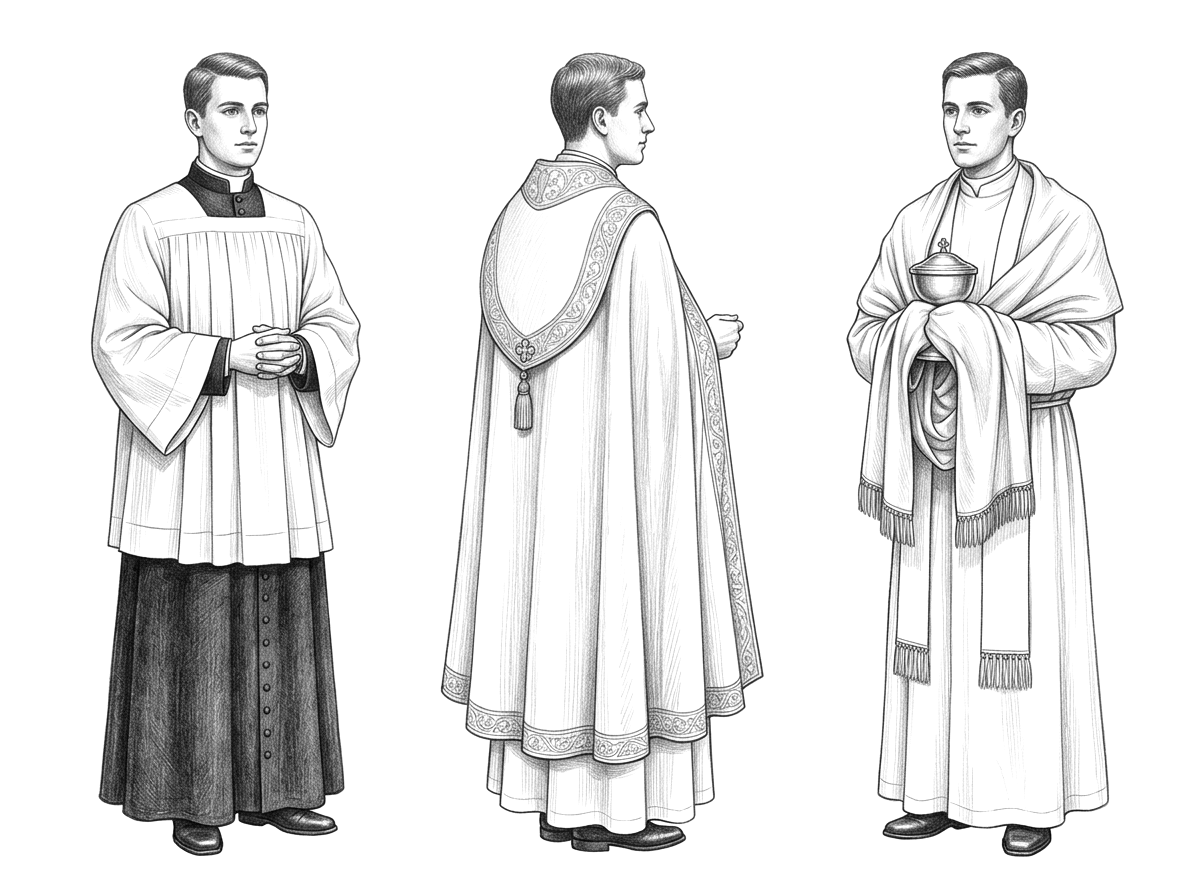
\includegraphics[width=0.92\linewidth,height=3.55in,keepaspectratio]{liturgy/roman-rite/postconciliar/2008-latin-2011-us-english/reference/roman-sanctuary-dictionary/shared/artwork/graphite/pc-art-09-black-cassock-surplice-cope.png}
\end{center}
\PCDPositionKey{Left: choir dress (deep black buttoned clerical Cassock beneath crisp white pleated Surplice); center: three-quarter rear view of semicircular Cope with ornamental hood shield and tassel over an Alb; right: Priest in Alb and straight Stole wearing a fringed Humeral Veil whose cloth completely envelops both hands supporting a closed lidded ciborium.}
\else
\textbf{Visual Plate Summary (Plate IX --- Choir Dress and Solemn Ceremonial Vesture, Standing figures to common scale):} Three-figure monochrome graphite garment study demonstrating high-contrast shading: left, a standing figure in clerical choir dress wearing a deep charcoal-black ankle-length buttoned cassock under a bright white pleated wide-sleeved surplice; center, three-quarter rear view of a flowing semicircular cope with embroidered hood shield and tassel worn over a white alb; right, three-quarter front view of a priest in alb and straight vertical stole draped in an oblong fringed humeral veil whose ends wrap completely over both hands as he holds a closed lidded ciborium.

\textbf{Reading order and object placement:} Left: choir dress (deep black buttoned clerical Cassock beneath crisp white pleated Surplice); center: three-quarter rear view of semicircular Cope with ornamental hood shield and tassel over an Alb; right: Priest in Alb and straight Stole wearing a fringed Humeral Veil whose cloth completely envelops both hands supporting a closed lidded ciborium.
\fi

\label{pc-obj-cassock-surplice}
\PCDEntryHead{Cassock and Surplice}{Vestis talaris et superpelliceum}{permitted}{N37}
\PCDField{Also called}{Choir Dress; Server's Cassock and Surplice; \textit{Talaris}; \textit{Superpelliceum}; \textit{Cotta}}
The cassock and surplice pair an ankle-length buttoned dark robe with a knee- or hip-length pleated white linen over-tunic, worn by non-concelebrating clergy in choir dress and---as a lawful dignified alternative to the alb---by altar servers. Rendered on the left figure of Plate IX in clerical choir dress: a deep charcoal-black buttoned cassock reaching the ankles beneath a crisp, bright white square-yoked pleated surplice with wide open sleeves.

\PCDField{Plate position and status}{Left figure, deep charcoal-black ankle-length buttoned cassock under bright pleated white surplice (Plate IX) (Universal Roman law)}
\PCDField{Placement and liturgical use}{In postconciliar discipline, two sharp rules govern cassock and surplice. First, the alb may never be exchanged for a surplice, not even over a cassock, when a chasuble or dalmatic is worn or when rubrics prescribe only a stole without an outer vestment (GIRM 336; CE 1984 no. 65). Second, whenever a surplice is worn, it must always be worn over a cassock---never directly over ordinary street clothing (CE 1984 no. 65). Non-concelebrating priests attending Mass in choir wear choir dress or a surplice over a cassock (Redemptionis Sacramentum 128). For altar servers in the United States, cassock and surplice remain a widely esteemed, dignified traditional alternative to the white alb (US GIRM 339).}
\PCDField{United States norm}{Under the United States adaptation to GIRM 339, altar servers, acolytes, readers, and other lay ministers may wear either the alb or other appropriate and dignified clothing such as cassock and surplice. Universal law strictly forbids substituting a surplice over a cassock for the alb whenever a chasuble, dalmatic, or stole alone is worn (GIRM 336), and requires that a surplice always be worn over a cassock (Caeremoniale Episcoporum 1984 no. 65).}
\PCDField{Ministers and server boundary}{Ordinary ministers: Bishop, Priest, Deacon, Instituted acolyte, Altar server. Server handles directly: Altar servers wear cassock and surplice where parish custom appoints them (US GIRM 339), always wearing the surplice over a properly fitted cassock (never over street clothes alone) and never adding clerical collars, stoles, or prelatial insignia.}
\PCDSafety{Ensure the cassock hem clears the floor cleanly above the shoes so it does not catch on sanctuary steps while carrying candles, the processional cross, or a smoking thurible; never wear a surplice without a cassock underneath (CE 1984 no. 65).}
\PCDField{Distinguish from}{Alb}
\PCDField{1962 Roman Missal counterpart}{\PCDTag{changed use} In the 1962 Roman Missal, cassock and surplice were the standard vesture of altar servers, choir clergy, and priests administering many non-Mass rites with a stole (RS II.1, VI.8). Postconciliar GIRM 336 replaces surplice-and-stole with alb-and-stole whenever rubrics prescribe a stole alone or beneath chasuble/dalmatic, while retaining cassock and surplice for choir dress (RS 128) and permitting them for altar servers alongside the alb (US GIRM 339; CE 1984 no. 65).}
\PCDEntryRule

\label{pc-obj-cope}
\PCDEntryHead{Cope}{Pluviale}{provided}{N38}
\PCDField{Also called}{Processional Mantle; \textit{Cappa}}
The cope is a long, open-fronted semicircular ceremonial mantle fastened across the chest with a clasp (morse), worn by a bishop, priest, or presiding deacon in processions, Solemn Vespers, Eucharistic Benediction, and other non-Mass rites. Shown on the center figure of Plate IX in three-quarter rear view over a white alb: a sweeping floor-length semicircular cloak bordered with ornamental trim and carrying a flat, shield-shaped decorative hood finished with a single tassel across the upper back.

\PCDField{Plate position and status}{Center figure, three-quarter rear view showing full semicircular cloak, embroidered hood shield, and tassel over an alb (Plate IX) (Universal Roman law)}
\PCDField{Placement and liturgical use}{GIRM 341 specifies that the cope is worn by the priest in processions and during other sacred actions in accordance with the rubrics proper to individual rites---such as Solemn Benediction with the monstrance (where a white cope and humeral veil are prescribed: Holy Communion and Worship of the Eucharist Outside Mass nn. 91--92), Eucharistic processions, Solemn Liturgy of the Hours, solemn blessings, and funeral rites outside Mass. A priest never celebrates the Mass itself in a cope: if worn for an entrance procession such as Palm Sunday, he exchanges it for the chasuble before beginning the Mass prayers (GIRM 337, 341). A deacon wears the cope only when presiding at specific non-Mass rites such as Solemn Benediction or Solemn Vespers.}
\PCDField{United States norm}{GIRM 341 governs the cope universally according to the rubrics of individual rites; United States GIRM 346e and 346h apply to funeral and festive gold/silver color choices.}
\PCDField{Ministers and server boundary}{Ordinary ministers: Bishop, Priest, Deacon. Clergy-reserved; server does not touch: Strictly reserved to bishops, priests, and deacons presiding at proper non-Mass rites; servers never wear a cope, though servers may assist in vesting it in the sacristy and---when directed during Benediction or processions---hold back its front edges as the celebrant incenses or blesses.}
\PCDSafety{When holding the edges of a priest's or bishop's cope during incensation or procession, keep the heavy front fabric well clear of lighted candles and hot thurible chains, and unfasten the chest clasp gently without tugging delicate embroidery.}
\PCDField{Distinguish from}{Chasuble, Humeral Veil}
\PCDField{1962 Roman Missal counterpart}{\PCDTag{continued} The cope continues from 1962 usage in processions, solemn Office, and Eucharistic Benediction (GIRM 341; HCWEOM nn. 91--92). Following Tres abhinc annos (1967) no. 26 and GIRM 51 and 337, postconciliar rubrics permit the chasuble rather than requiring a cope for rites integrated directly into Mass such as the Sunday sprinkling rite and Ash Wednesday imposition of ashes.}
\PCDEntryRule

\label{pc-obj-humeral-veil}
\PCDEntryHead{Humeral Veil}{Velum humerale}{provided}{N39}
\PCDField{Also called}{Benediction Veil; \textit{Velum}}
The humeral veil is a long oblong fringed white cloth draped across the shoulders and fastened across the chest so that its ends completely envelop the hands of the bishop, priest, or deacon when holding the monstrance or ciborium during Eucharistic Benediction and processions. Shown on the right figure of Plate IX over an alb and straight priestly stole: a broad rectangular white shawl with fringed ends fastened in front, whose generous fabric wraps completely around both hands holding a closed lidded ciborium---never leaving bare hands gripping the vessel.

\PCDField{Plate position and status}{Right figure, oblong fringed white cloth draped over shoulders with ends wrapping completely over both hands around a lidded ciborium (Plate IX) (Universal Roman law)}
\PCDField{Placement and liturgical use}{The Eucharistic humeral veil is required whenever a bishop, priest, or deacon imparts Benediction with the monstrance (over a white cope) or with a ciborium, carries the Blessed Sacrament in a solemn procession (such as Corpus Christi), or transfers the Blessed Sacrament to the altar of reposition at the close of the Holy Thursday Evening Mass of the Lord's Supper (Holy Communion and Worship of the Eucharist Outside Mass nn. 91--92; Roman Missal, Holy Thursday). Extraordinary ministers of Holy Communion and altar servers never impart Eucharistic Benediction and never wear the Eucharistic humeral veil. Distinguish the Eucharistic humeral veil from the narrower vimpa worn by miter- and crosier-bearers during pontifical liturgies (Caeremoniale Episcoporum 1984).}
\PCDField{Ministers and server boundary}{Ordinary ministers: Bishop, Priest, Deacon. Server carries and presents to priest or deacon: Servers never wear the Eucharistic humeral veil to carry or bless with the Blessed Sacrament. During Benediction or Holy Thursday transfer, a server places the humeral veil evenly across the priest's or deacon's shoulders, fastens the front clasp securely, and removes and folds it cleanly afterward.}
\PCDSafety{Fasten the front clasp cleanly and evenly without pulling the priest's stole or collar, and ensure the long fringed ends do not brush against lighted candles on the altar steps while the celebrant ascends to lift the monstrance or ciborium.}
\PCDField{Distinguish from}{Cope, Stole}
\PCDField{Symbolism}{Covering the minister's hands in clean white cloth while raising the monstrance or ciborium expresses profound reverence before Christ's Real Presence and visibly manifests that Christ Himself---not the human minister---imparts the Eucharistic blessing. (Holy Communion and Worship of the Eucharist Outside Mass (1973) nn. 91--92; Roman Missal (2008/2011), Evening Mass of the Lord's Supper)}
\PCDField{1962 Roman Missal counterpart}{\PCDTag{changed use} In the 1962 Roman Missal, the humeral veil served both Eucharistic Benediction and processions and---at Solemn High Mass---the subdeacon, who wore it from Offertory to the Pater Noster to hold the empty paten (RS VII.9, X.8). After Paul VI's Ministeria quaedam (1972) suppressed the subdiaconate and the 1969/1970 Order of Mass omitted subdiaconal paten-holding, the humeral veil's liturgical use is dedicated exclusively to Eucharistic Benediction, processions, and Holy Thursday transfer.}
\PCDEntryRule
